% ---------
%  Compile with "pdflatex hw1".
% --------
%!TEX TS-program = pdflatex
%!TEX encoding = UTF-8 Unicode

% Template borrowed from Jeff Erickson.

\documentclass[11pt]{article}
\usepackage[utf8]{inputenc}		% Allow some non-ASCII Unicode in source
\usepackage{jeffe, handout,graphicx}
\usepackage{forest}
\usepackage{mathtools}
\usepackage{tikz, ifthen, etoolbox}
\usepackage{float}
\usetikzlibrary{positioning}
\newcommand{\pd}{\partial}
\newcommand{\bs}{\boldsymbol}
\newcommand{\ifstringequal}[4]{%
  \ifnum\pdfstrcmp{#1}{#2}=0
  #3%
  \else
  #4%
  \fi
}


% =========================================================
%   Define common stuff for solution headers
% =========================================================
\Class{CS 6301.503}
\Semester{Spring 2019}
\Authors{1}
\AuthorOne{Scott C. Waggener}{scw180000}
%\Section{}
% =========================================================
\begin{document}
\HomeworkHeader{4 (Probability)}{1}% homework number, problem number
% ---------------------------------------------------------
Complete

% =========================================================
\HomeworkHeader{4 (Probability)}{2}% homework number, problem number
% ---------------------------------------------------------
Complete

% =========================================================
\HomeworkHeader{4 (Probability)}{3}% homework number, problem number
% ---------------------------------------------------------
\noindent
\begin{enumerate}[(a)]\itemsep0pt
\item You're person B and want to win, which version of the game do you play?
	\begin{solution}
		The standard version
	\end{solution}

	\begin{proof}
		First a qualitative answer: In the standard version of the game
		answers are received immediately after each question, meaning that the
		answer to question $q-1$ will inform what should be asked for question
		$q$. Expressed mathematically, the conditional probability of possible
		objects at iteration $i$ will be of the form

		\begin{align}
			P(O=o_n) = P\bigg(o_n \Big\vert a_{i-1}, a_{i-2}, \dots a_{1}\bigg)
		\end{align}

		where $a_i$ is the answer to the $i$th question. If person B wants to
		maximize $P(O=o_n)$ for some object, they need
	\end{proof}
\end{enumerate}

% =========================================================
\HomeworkHeader{4 (Probability)}{4}
% ---------------------------------------------------------
\begin{solution}
	The plot was generated using $100$ trials for each of the possible number
	of known questions. Sampling was done using $\texttt{np.random.binomial}$
	with $n=1,\ p=0.25,\ \text{size}=(100 - \text{known})$
	\begin{figure}[H]
		\centering
		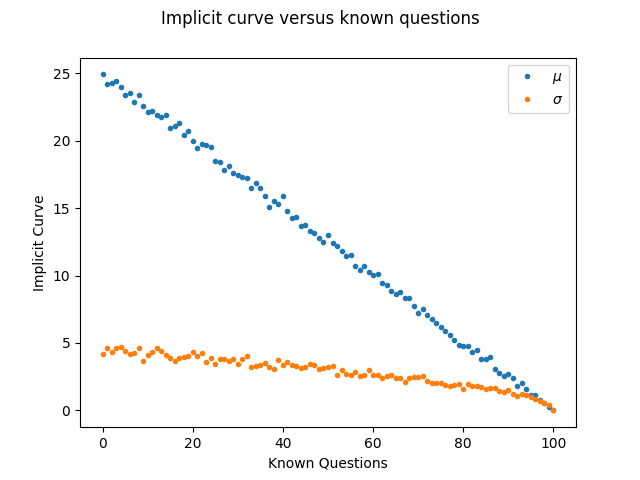
\includegraphics[width=0.8\linewidth]{figures/q4.png}
		\caption{Implicit curve $\mu, \sigma$ versus number of known questions.}
	\end{figure}

\end{solution}


% =========================================================
\HomeworkHeader{4 (Probability)}{5}
% ---------------------------------------------------------
Assume ImageNet has 1.28 million images of size 3 x 256 x 256 with 1280 images
each in 1000 different classes. How many bits of information are in the ImageNet
labels?

\begin{solution}
	$10$ bits
\end{solution}

\begin{proof}
	Since entropy can informally be defined as the information in the
	realization of a random variable, we can compute the entropy for the given
	problem. We have $1280$ images in each of the $1000$ classes, meaning
	\begin{align}
		H(x(s)) &= -\Sum_{i=1}^{1000} \frac{1}{1000}\log_2\left(
			\frac{1}{1000}\right)
		\\
		&= -\frac{1000}{1000} \log_2\left(\frac{1}{1000}\right)
		\\
		&= \log_2 1000
		\\
		&\approx 9.97
	\end{align}
\end{proof}


\end{document}
